\documentclass{jlreq}

\usepackage{listings}
\usepackage{caption}
\usepackage{fancyhdr}
\usepackage{graphicx}

\lstset{
    language=C, % 使用するプログラム言語を指定
    basicstyle=\ttfamily\footnotesize, % フォントの指定
    numbers=left, % 行番号を表示(必要な場合)
    numberstyle=\tiny, % 行番号のスタイル
    frame=single, % ソースコードを枠で囲む(必要な場合)
    breaklines=true, % 長い行を自動的に折り返す
    captionpos=b, % キャプションの位置を下にする
}
\renewcommand{\lstlistingname}{ソースコード}

\pagestyle{fancy}
\fancyhf{} % 既存のヘッダーとフッターをクリア
\fancyhead[R]{\thepage}% 右上にページ番号を配置
\setlength{\headheight}{17.0pt}
\addtolength{\topmargin}{-7.0pt}

\begin{document}

\tableofcontents
\clearpage

\section{実験機材}

マイコンボードの通し番号:\ 72

使用したパソコン:\ Lenovo Ideapad slim 550(持ち込み)

OS:\ Windows11 Home

\section{理論}

\subsection{PWM}
PWMは,周期一定の矩形波を出力し続けながら,パルス幅を変化させる機能である.
本実験においては,サーボモーターの制御に用いられる.LaunchPadには最大16個のPWM波形を生成する機能があり,
各波形を自由に調整することができる.PWMは2系統存在し,各系統別に4つのPWM生成器を持っている.各生成器は2本の出力ピンを制御することができ,
内蔵RGB LEDを制御するためにはピンの割り当てを適切に行う必要がある.

\subsection{I$^2$C}
I$^2$Cは,低速な周辺機器をマザーボードへ接続するのに用いられる通信規格である.
SCL(クロック)とSDA(データ)の2本の信号線によるシリアル通信であり,この信号線上に複数の機器を接続することができる.
複数の周辺機器は異なるアドレスが付与され,通信の最初にアドレスを指定する.送信と受信は同時に行わず時分割する.
通信速度は遅いため高速に大量のデータをやりとりするような用途には向かないが,
信号線の本数を劇的に削減できるメリットがあるため,速度の要求されない表示パネルなどに利用される.

\subsection{マイコンボード}
本実験で扱うボードは,Tiva C Series LaunchPadのEK-TM4C123GXLというボードである.
このボードには80MHzで動作するプロセッサ,256KBのフラッシュメモリ,32KBのSRAMが搭載されており,各種I/Oを制御することができる.
また,システムクロックには16MHzの水晶発振器を利用している.主な機能はすべて中央のプロセッサに内蔵されており,プロセッサから利用できるピンを
周囲のヘッダに引き出した形になっている.

\subsection{LED}
LaunchPadには3色LEDが内蔵されており,このLEDはGPIOポートFに接続されている.LEDを点灯させるには割り当てられたGPIOピンにH(1)を,
消灯するにはL(0)を出力する.また,PWMの制御によってLEDの光量や色合いを変えられる.

\subsection{ブザー}
圧電ブザーはGPIOピンに接続されており,PWM機能を利用して周期的にON-OFFを繰り返すパルス波形を出力することによって音を鳴らす.
一般的な音階の周波数$f$は次の式で与えられる.
\begin{equation}
    f=440\times2^{\frac{n}{12}}
\end{equation}
nの値を-9から+3と変化させることで音階を表せる.また,ブザーのONとOFFの時間を同じにするためにはパルス幅を周期の半分として与えるなど,
様々な工夫をすることで多種多様な音を表すことができる.

\subsection{LCD}
LCDとはキャラクタ液晶ディスプレイのことである.
LCDを周辺機器として接続し,LCDのアドレスに適切な命令とデータをI$^2$Cバスに流すことでLCDの設定や文字情報を制御することができる.

\section{実験内容}

\subsection{【課題1】仮想シリアルポートへの出力}
指定のプロジェクトをCCSにインポートした.そして,仮想シリアルポートへの出力をTerminal Pluginによって受信するために,以下のように設定した.
\begin{figure}
    \centering
    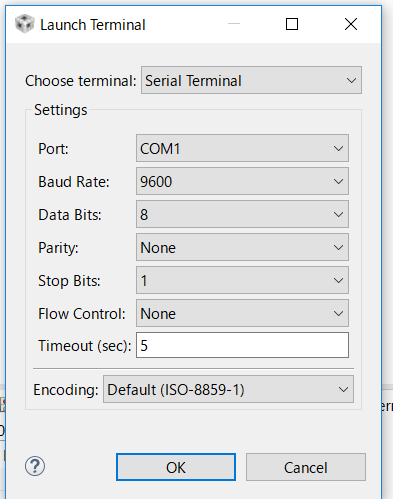
\includegraphics[width=0.3\textwidth]{setting_virtual_serial_port.png}
    \caption{Terminal Pluginの設定}
    \label{fig:Terminal_Plugin}
\end{figure}
この設定の後,blinky\_main.cのmain()関数内のUARTprintf()のコメントアウトを外してビルドを行った.

\subsection{【課題2】blinkyの改造}
blinky\_main.cのmain()関数内でGPIO割り込みを有効化し,initInterruptPins()関数とSW1PinIntHandler()関数を実装し,
SW1の割り込みによってLEDの点灯色を変化させるプログラムに改造した.また,このとき初期状態で有効化されていたSystickの割り込みを無効にした.

\subsection{【課題3】buzzerの改造}
まず,未完成のbuzzer.cにおいて,音階を表す変数を受け取ってその音を鳴らすtoneBuzzer()関数と,
呼び出すことで音が鳴り止むrestBuzzer()関数を実装した.そして,blinky\_main.cでinitInterruptPins()関数を実装し,
SW1PinIntHandler()関数にてSW1を押すことで音を鳴らしたり消したりするのに加えて,押した回数に従って「ド」から音階を上げて
規定回数以降にまた「ド」に戻るようにプログラムを改造した.

\subsection{【課題4】setAddressLCD()関数とwriteTextLCD()関数の実装}
lcd\_SB1602.cに,LCDの文字位置を指定するsetAddress()関数と,LCDへの文字表示を実行するwriteTextLCD()関数を実装した.
そして,lcd\_main.cで直書きされている文字位置の指定と文字表示の実行のコードをsetAddress()とwriteText()を使うように改造した.

\subsection{【課題5】SW1を押した回数のLCDへの表示}
まず,initInterruptPins()関数を実装し,SW1PinIntHandler()関数を,Systickに割り込みを無効化した後にSW1の押下によって
カウントが実行されてLCDへカウント文字列を表示するように実装した.また,main()関数内でGPIO割り込みを有効化した.

\section{実験結果}

\subsection{【課題1】仮想シリアルポートへの出力}


\subsection{【課題2】}
以下に,initInterruptPins()のソースコードを示す.

\begin{lstlisting}[label=src1,caption={initInterruptPins()}]
void initInterruptPins(void) {
    // Clear Interrupt
    GPIOIntClear(GPIO_PORTF_BASE,INT_ALL_BUTTONS);

    // Register a handler function
    GPIOIntRegister(GPIO_PORTF_BASE,SW1PinIntHandler);

    // Set type of interrupt to falling edge
    GPIOIntTypeSet(GPIO_PORTF_BASE,INT_ALL_BUTTONS,GPIO_FALLING_EDGE);
}
\end{lstlisting}

この関数内では,3行目にポートFに接続された全てのスイッチによる割り込みの処理を完了させ,
6行目でポートFにSW1PinIntHandler関数を割り当てて割り込みハンドラを指定し,
9行目でSW1が押されたとき,すなわち波形がL(0)のときに割り込みが発生するように設定した.

次に,SW1PinIntHandler()のソースコードを示す.

\begin{lstlisting}[label=src2,caption={SW1PinIntHandler()}]
void SW1PinIntHandler(void) {
    disableSW1PinInt();
    // Clear Interrupt
    clearSW1PinInt();
    SysTickIntDisable();

    GPIOPinWrite(GPIO_PORTF_BASE,base_led_color,0);

    int light[]={LED_BLUE,LED_RED,LED_GREEN,LED_WHITE};
    static int cnt=0;
    base_led_color=light[(++cnt)%4];
    GPIOPinWrite(GPIO_PORTF_BASE,base_led_color,led_color);

    enableSW1PinInt();
}
\end{lstlisting}

この関数内では,2行目に新たなSW1の押下による割り込みを防ぎ,
4行目でSW1による割り込みの処理を除去した.
そして,6行目でLEDを一旦消灯させて,8行目から11行目にかけてLEDを点灯させるコードを加えた.初期状態が青でそこから赤,緑,白,青となるように,LEDの色を表すマクロ定数を配列に格納し,
static宣言されたカウント用変数cntの値に応じて色を選択するようにした.
これらの処理を終えたあと,13行目でSW1の押下による新たな割り込みを許可した.

\subsection{課題3}

\subsection{課題4}

\subsection{課題5}

\section{考察}

\section{問題回答}

\end{document}